\documentclass[
	parskip=half,10pt,
	numbers= noenddot, % enddot -> Ebenen mit Punkt abschließen -> 1.1., noenddot -> ohne Punkt
	toc=flat, % TOC in Tabellenform (bei langen Überschrtiften verwenden)
	oneside,
	twocolumn,
	]{scrartcl}



\usepackage[T1]{fontenc} % verwende Type 1 - Zeichensatz
\usepackage{libertine}
\usepackage[scaled=0.78]{beramono} %Schreibmaschinenschrift
\usepackage{microtype}
\usepackage[utf8]{inputenc}
\usepackage[ngerman]{babel} % internationale Sprachunterstützung



\usepackage{amsmath}
\usepackage{amssymb}
\usepackage{amsthm}
\usepackage{tabularx}
\usepackage{booktabs}
\usepackage{longtable}
\usepackage{rotating} % Rotationen, Reflexionen, ...
\usepackage{multido} % Wiederholungen
\usepackage{wrapfig}
\usepackage{todonotes}
\usepackage{siunitx} %\si units
\usepackage{units}
\usepackage{icomma} %keine Leerzeichen nach Komma im mathmode
\usepackage[numbers,sort]{natbib}
\usepackage{babelbib}%deutsche bibliographie
\usepackage{multirow}
\usepackage{rotating}
\usepackage{url}
\usepackage{float}
\usepackage{tikz}
%\usetikzlibrary{external}
%\tikzexternalize
%\tikzsetexternalprefix{figs/}

\usepackage{pgfplots}
\pgfplotsset{compat=1.8}
\usepackage{placeins}
\usepackage{caption}
\usepackage{graphicx}
\usepackage{subcaption} %für subfigures
\captionsetup{labelfont={bf,sf},format = plain, textfont=sf}
%\usepackage{asymptote}
\usepackage{ragged2e}
\usepackage[bottom]{footmisc}
\usepackage{csquotes} %Anführungszeichen
\usepackage[ngerman]{varioref} % Zum komfortablen Verlinken



\usepackage{geometry}
\geometry{a4paper,lmargin=2.5cm, rmargin=2.5cm, tmargin=2.5cm, bmargin=3cm, marginparwidth=3cm, marginparsep=1em}


\usepackage{fancyhdr}
\pagestyle{fancy}
\renewcommand\footrulewidth{0.5pt}
\fancyhf{}
\lhead{\leftmark}

\fancyfoot{}
\rfoot{\thepage}
\lfoot{Till Kolster \& Lukas Schmidt}


\usepackage{layout}

\usepackage[%draft
linkbordercolor=blue,
colorlinks,
linkcolor=blue,
linktocpage,
linktoc=all]{hyperref} % IMMER AM ENDE

%\setkomafont{subparagraph}{\mdseries\itshape}
\setcounter{secnumdepth}{3}%Bis zu welcher Ebene nummeriert werden soll. 
\setcounter{tocdepth}{2}%Bis zu welcher Tiefe ins TOC soll.

%%%%%EIGENE DEFINITIONEN%%%%%

\newcolumntype{Y}{>{\RaggedRight\hspace{0pt}} X }
\newcommand\Grad{$^\circ$}
\newcommand\HAND{\marginnote{\Large\vreflectbox{\ding{43}}}\xspace}%\newcommand\Name{Befehlsdifinition}
\newcommand\MPAR[1]{
\marginnote[\RaggedLeft#1]{\RaggedRight#1}}
% \hspace{0pt} entspricht dem ersten (nicht sichtbaren) Wort
\newcolumntype{P}[1]{>{\RaggedRight\hspace{0pt}}p{#1}}
\newcolumntype{R}{>{\tiny}r}

\pgfmathdeclarefunction{gauss}{4}{%
  \pgfmathparse{#1*exp(-((x-#2)^2)/(2*#3^2))+#4}%
}


\title {Rayleigh-Scattering}
\author {Till Kolster \thanks{Freie Universität Berlin} \and Lukas Schmidt \thanks{Freie Universität Berlin}}


\begin{document}

\begin{titlepage}

\vspace*{-2cm}

\vspace{6cm}
\begin{center}
\huge \bfseries
Fortgeschrittenen-Praktikum -- Gamma-Spektroskopie

\vspace{0.5cm}
\large \bfseries
\today

\vspace{1.5cm}

\large\normalfont von

\bigskip
\textbf{Till Kolster \& Lukas Schmidt}

\bigskip
Tutor: Dr. Katayoun Gharagozloo-Hubmann

\vspace{3cm}

\parbox{0.8\linewidth}{%
\textit{Der Versuch wurde im Rahmen des Forgeschrittenenpraktikums am Fachbereich Physik der FU-Berlin durchgeführt und soll praktische Erfahrung und eine 
theoretische Vertiefung zu den kernphysikalischen Hintergründen von Radioaktivität und deren Messung geben.}}


\end{center}
\end{titlepage}


\section{Theoretische Grundlagen}

\subsection{Einleitung}

Radioaktive Strahlung hat verschieden Quellen, die wohl bekannteste ist der Zerfall von instabilen Atomkernen. Dabei treten verschiedene Strahlungsarten auf, 
die aus vielfältigen Gründen gemessen und quantifiziert werden wollen. So kann eine gesundheitliche Belastung durch Strahlungsquellen von Interesse sein, die 
Aktivität dieser zu bestimmen. Im folgenden Versuch steht die Gammastrahlung als eine der drei Strahlungsarten im Fokus.  

\subsection{Kernzerfälle}

Radioaktiver Kernzerfall kann auf verschiedene Arten stattfinden, $\alpha, ~\beta, ~ \gamma$-Zerfall genannt. Auf sogenannten Nuklidkarten wird aufgezeichnet, welche 
Isotope eines Atoms mit welcher Strahlungsart zerfallen. Die Einteilung in $\alpha, ~\beta, ~ \gamma$-Strahlung folgt der Wechselwirkung der Strahlung mit Materie.

\subsubsection{$\alpha$-Zerfall}
Beim $\alpha$-Zerfall verringert das Atom seine Kernladungszahl um den Betrag zwei, indem es einen ionisierten Helium-4-Kern verliert. Dieser Helium-Kern wird in diesem 
Zusammenhang als $\alpha$-Teilchen bezeichnet. Da die kinetische Energie des Teilchens charakteristisch für den $\alpha$-Strahler ist, kann die Bestimmung dieser 
Energie dazu dienen, den Strahler zu identifizieren. Da das zurückbleibende Tochternuklid nun einen Elektronenüberschuss besitzt, werden diese an die Umgebung abgegeben 
\cite{kuckuk}. 


\subsubsection{$\beta$-Zerfall}
$\beta$-Zerfall bezeichnet die Emittierung von Elektronen ($\beta^-$) und Positronen ($\beta^+$) durch einen Atomkern. Gleichzeitig emittiert der Kern ein 
Antineutrino oder ein Neutrino ($\beta^+$). Dabei wird ein Neutron zum Proton umgewandelt bzw. andersherum wenn es sich um den $\beta^+$-Zerfall handelt. Die 
Massenzahl des Atoms bleibt bei diesem Prozess gleich, die Kernladungszahl wird jedoch um 1 vergrößert bzw. verkleinert ($\beta^+$). 

Wenn ein Proton des Atomkerns ein Elektron einfängt, verwandelt es sich zu einem Neutron und einem Neutrino. Dieser Prozess wird Elektroneneinfang genannt.
Die Emittierung eines Positrons kann nur zusammen mit diesem Prozess stattfinden, der Elektroneneinfang kann jedoch auch unabhängig stattfinden. Die 
freiwerdende Energie kann komplett an das freigesetzte Neutrino abgegeben werden oder verbleibt (zum Teil) im Kern und kann als $\gamma$-Strahlung abgegeben werden. 
Außerdem wird das entstandene Loch in der Schale, aus der das Elektron eingefangen wurde wieder aufgefüllt. Die hierbei frei werdende Energie kann entweder 
in Form eine Augerelektrons oder als Röntgenstrahlung emittiert werden. 

\subsubsection{$\gamma$-Zerfall}

Als Gammastrahlung werden Photonen mit Energien von mehr als $300 \si{\kilo \electronvolt}$ bezeichnet, oder elektromagnetische Strahlung, die einem Kern 
entstammt oder deren Ursprung nicht bekannt ist. Davon abgegrenzt ist die Röntgenstrahlung, die durch Elektronenprozesse hervorgerufen wird und im Bereich von 
ca. $100-300 \si{\kilo \electronvolt}$ liegt. 

Im Gegensatz zum $\alpha$- und $\beta$-Zerfall, ändert sich bei dieser Strahlungsart weder Massenzahl noch Kernladungszahl. Sie ist allein auf das Abregen eines 
angeregten Zustandes des Kerns zurückzuführen. Diese Relaxation folgt manchmal den beiden anderen Zerfallsarten. Gamma-Strahlung kann jedoch auch auf andere 
Weise entstehen, beispielsweise durch die sogenannte Paarvernichtung. 

\subsection{Photoeffekt}

Ein Prozess, bei dem Materie mit hochenergetischer Strahlung wechselwirkt ist der Photoeffekt. Dabei gibt ein Photon bei einem Absorptionsprozess seine gesamte Energie 
an ein Elektron ab \cite{schatz}. Die kinetische Energie des so emittierten Elektrons ist dann gleich der des Photons minus der Bindungsenergie aus dem Atom. Diese 
Bindungsenergie verbleibt zunächst im Atom und kann in Form eines Auger-Elektrons oder Röntgen-Strahlung abgegeben werden. Der Wirkungsquerschnitt 
des Photoeffekts kann folgender Näherung entnommen werden:

\begin{align}
\sigma_{Ph} &\propto E^{-3,5}_{\gamma} \cdot Z^5,
\end{align}
Mit $E_{\gamma}$ der Energie des einfallenden Photons und $Z$ der Kernladungszahl des einfangenden Atoms. Elemente mit hoher Kernladungszahl erreichen daher die 
beste Abschirmung der Primärstrahlung pro Dicke des Materials. Es empfiehlt sich also zur Abschirmung gegen hochenergetische 
Strahlung Elemente mit hoher Kernladungszahl zu benutzen, jedoch entstehen relativ große Mengen an Sekundärstrahlung, die unter Umständen eine stärkere 
Wechselwirkung mit beispielsweise organischen Materialien zeigen.  


Mit steigender Energie des Photons nimmt jedoch der Wirkungsquerschnitt ab, erreicht die Photonenenergie jedoch die Energie, die zum ionisieren der Schale, die in 
der Energieskala höher liegt, springt der Wirkungsquerschnitt wieder auf einen höheren Wert. Dies findet so lange statt, bis keine höherenergetischen Schalen mehr 
existieren, wie in Abbildung \ref{fig:absorption} zu sehen ist. 

\begin{figure}[h]
\centering
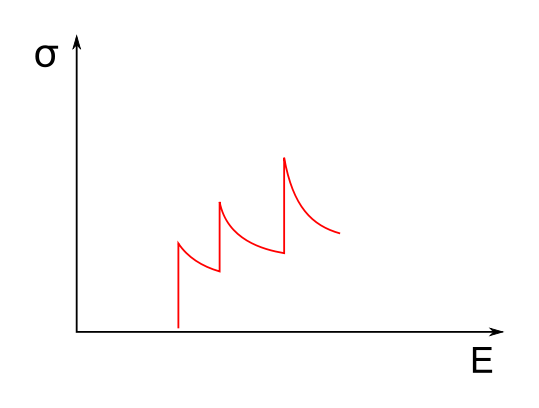
\includegraphics[width=.4\textwidth]{images/kante.png}
\caption{Schematischer Darstellung des Wirkungsquerschnittes als Funktion der Photonenenergie \cite{wikipedia}}
\label{fig:absorption}
\end{figure}

Die Sprungkanten werden als Absorptionskanten bezeichnet und sind im Absorptionsspektrum gut sichtbar. Der Photoeffekt ist also sehr wichtig bei kleineren Photonenenergien 
und Materialien mit hoher Kernladungszahl \cite{schatz}.

\subsection{Compton-Streuung}

Bei der Compton-Streuung wird nicht wie beim Photoeffekt die gesamte Energie auf eine Elektron übertragen, sondern nur ein Teil. Wie viel, hängt vom Winkel des 
Zusammenstoßes zwischen Photon und Elektron ab, es handelt sich also um einen elastischen Stoß. Das Elektron wird hierbei als frei angenommen, was bei den 
äußeren Elektronen eines Atoms näherungsweise stimmt. Durch den Energieverlust wird die Wellenlänge des Photons um den Betrag $\Delta \lambda$ vergrößert, für 
welche folgende Relation gilt:

\begin{align}
\Delta \lambda &= \frac{h}{m_e c} (1 - \cos \phi) = \lambda_c (1 - \cos \phi),
\end{align}
mit $\lambda_c$ der Compton-Wellenlänge, $m_e$ der Masse des Elektrons, $h$ dem Planckschen Wirkungsquantum, $c$ der Lichtgeschwindigkeit und $\phi$ dem Streuwinkel. 
Der Energieverlust hängt also allein vom Streuwinkel ab. 

Der Wirkungsquerschnitt ist somit allein von der Elektronendichte abhängig, welche ungefähr proportional zur Kernladungszahl ist. Somit ergibt sich für 
den Wirkungsquerschnitt folgende Näherung: 

\begin{align}
\sigma_C &\propto E_{\gamma}^{-1} \cdot Z
\end{align}

Der Comptoneffekt stellt sich somit als besonders wichtig heraus für mittlere Energien zwischen $100$ und $1000 \si{\kilo \electronvolt}$. 

Wenn nun die gestreuten Photonen energieaufgelöst beobachtet werden, so ist die Energie des gestreuten Photons $E_{\gamma}'$ in Abhängigkeit des Winkel von Interesse:
\begin{align}
E_{\gamma}'(\phi) &= \frac{E_{\gamma}}{1 + \frac{E_{\gamma}}{m_e c^2} (1 - \cos \phi)}
\end{align}

Bei Aufnahme eines Spektrums ergibt sich nun also ein kontinuierliches Spektrum für alle Winkel zwischen 0\textdegree und 180\textdegree. Danach folgt eine 
scharfe Kante, die sogenannte Compton-Kante, die auftritt, weil nicht mehr Energie abgegeben werden kann, als bei einem Stoß von 180\textdegree. Die 
korrespondierende Energie beträgt dann also 
\begin{align}
E_{\gamma}'(180^{\circ}) &= \frac{E_{\gamma}}{1 + \frac{2 E_{\gamma}}{m_e c^2}}
\end{align}

Zusätzlich sollte ein Maximum mit höherer Energie im Spektrum auftreten, da auch einige Photonen ohne Streuprozess durch das Material fliegen. Dieses Maximum wird 
Photopeak genannt. Zu jedem Photopeak gibt es also eine korrespondierende Compton-Kante. 

\subsection{Paarbildung/-vernichtung}

Bei höheren Photonenenergien von ab $1022 \si{\kilo \electronvolt}$ tritt als zusätzlicher Effekt die Paarbildung bzw. -vernichtung auf. Hierbei kann sich ein Photon 
im Feld eines Atomkerns oder eines Hüllenelektrons in Elektron und Positron aufspalten. 

Findet diese Aufspaltung im Feld eines Atomkerns statt, so geht fast die gesamte Energie des Photons in die beiden Teilchen über, davon $E = m_e c^2 = 511 
\si{\kilo \electronvolt}$ in die Ruhemasse jedes Teilchens und der Rest in die kinetische Energie. Elektron und Postiron fliegen dabei genau in entgegengesetzte Richtungen 
senkrecht zur Bahn des erzeugenden Photons, sodass der Impuls beider Teilchen zusammenaddiert genau null ergibt. Da dem Photon ebenfalls ein Impuls zugeschrieben werden 
kann, der durch die beobachtbaren Bahnen nicht an die beiden Spaltprodukte übergegangen sein kann, muss dieser an den beteiligten Atomkern übergehen und beträgt 
$p=\nicefrac{E_{\gamma}}{c} = \nicefrac{h \nu}{c}$. 

Trifft nun ein Elektron auf ein Positron, so kommt es zur Paarvernichtung, dabei werden jedoch zwei Photonen frei, die sich aufgrund der Impulserhaltung bei vorher 
ruhenden Teilchen in genau entgegengesetzte Richtungen bewegen. 
Wird die kinetische Energie des Elektrons und Positrons vernachlässigt, so besitzen beide Photonen eine Energie, 
die wieder genau der Ruheenergie eines Elektrons entstpricht, $511 \si{\kilo \electronvolt}$. Diese Energie kann im Detektor gemessen werden. Es kann jedoch auch 
vorkommen, dass ein Photon der Paarvernichtung aus dem Detektor entkommt. Dementsprechend verbleibt nur ein Teil der Energie des ursprünglichen 
Photons im Detektor. Wenn angenommen wird, dass das Elektron/Positron seine gesamte kinetische Energie im Detektor verloren hat, beträgt die Energie des 
sogenannten Single-Escape-Peaks $E = E_{\gamma} - 511 \si{\kilo \electronvolt}$. Entkommen das Paar, so fehlt dementsprechend doppelt so viel Energie: 
$E = E_{\gamma} - 1022 \si{\kilo \electronvolt}$. 

Paarbildung bzw. -vernichtung wird für hohe Photonenenergien zum dominierenden Effekt und ihr Wirkungsquerschnitt hat folgende Abhängigkeit \cite{harvey}:

\begin{align}
\sigma_A &\propto Z^2 \ln E_{\gamma}
\end{align}  


\subsection{Massenschwächungskoeffizient}

Um die Stärke der Interaktion von Gammastrahlung mit Materie zu beschreiben, wird ein Exponentieller Ansatz gewählt, in die drei vorgestellten Effekte eingepasst 
werden:

\begin{align}
I(s) &= I_0 e^{- \mu s},
\label{eq:abs}
\end{align}
wobei $I$ die Intensität in Abhängigkeit der durchquerten Strecke $s$ ist und $\mu$ der Absorptionskoeffizient. Dieser ist Abhängig von der Atomdichte des Absorbers $n$ 
in Anzahl pro Volumen und dem totalen Wirkungsquerschnitt \cite{marmier}:

\begin{align}
\mu &= n \cdot \sigma_{tot} = n \cdot ( \sigma_{Ph} + \sigma_C + \sigma_A)
\label{eq:sigma}
\end{align}

Aufgrund der verschiedenen $Z$- und $E_{\gamma}$-Abhängigkeiten, bietet sich die in Abbildung \ref{fig:absorption_2} gezeigte Abhähngigkeit des Absorptionskoeffizienten 
von der Photonenenergie.

\begin{figure}[h]
\centering
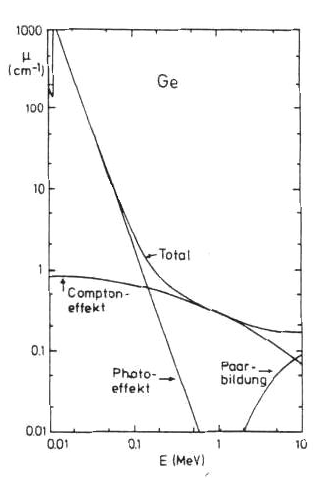
\includegraphics[width=.4\textwidth]{images/absorption.pdf}
\caption{Beitrag der verschiedenen Komponenten zum Absorptionskoeffizienten von Germanium \cite{schatz}}
\label{fig:absorption_2}
\end{figure}



\subsection{Szintillationsdetektor}

Der moderne Szintillationsdetektor oder -zähler beseht aus zwei Teilen: Dem Szintillator und dem Photomultiplier. Im Szintillator werden durch ionisierende Strahlung 
Exzitonen erzeugt. Diese ionisieren weitere Atome im Gitter. Energiereiche Strahlung erzeugt also mehrere Elektron-Loch-Paare. Diese rekombinieren nun wieder. 
Findet dies an den dotierten Störstellen statt, wird Energie in Form von Lichtblitzen frei \cite{kleinknecht}. Diese können mithilfe eines Photomultipliers 
festgestellt werden. Das Signal ist dann proportional zur Energie der detektierten Strahlung. Damit die Lichtblitze detektiert werden können, muss das Detektormaterial 
für sichtbares Licht durchsichtig sein. Daher ist der Szintillator 
häufig als Einkristall ausgeführt. Im Experiment wird als Material ein Thallium dotierter Natrium-Iodid Kristall verwendet. Das Thallium nimmt dabei den Platz der 
Natrium-Positionen im kubischen Kristallgitter ein. Je nach Dotierungskonzentration ändert sich die Auflösung des Detektors. 

\subsection{Halbleiterdetektor}

Ein Halbleiterdetektor besteht meist aus einem p-n-Übergang, bei dem ein positiv und ein negativ dotierter Halbleiter, in diesem Fall Germanium, aneinandergebracht werden. 
Fällt nun Strahlung in den Halbleiter ein, so erzeugt diese Elektron-Loch-Paare. Dies geschieht analog zum Szintillator durch anregung eines einzelnen Elektrons, 
welches dann auf seiner Bahn durch den Halbleiter weitere Elektronen anregt. Diese können abgegriffen und der erzeugte Strom oder die Schwankung in der Spannung gemessen 
werden. Die Anzahl der freigesetzten Elektronen wird dabei durch die Bandlücke bestimmt, da diese Energie zum anheben in das Leitungsband benötigt wird. Da diese 
Bandlücke nicht sehr groß ist, kann die Energie der Strahlung sehr gut aufgelöst werden. Um möglichst alle angeregten 
Elektronen abfangen zu können, wird eine Hochspannung angelegt, die die Elektronen absaugt und die Sperrschicht vergrößert. Außerdem wird der Detektor gekühlt, um 
eine thermische Anregung ins Leitungsband zu verhindern und um den Leckstrom gering zu halten, der bei der angelegten Hochspannung den Detektor zerstören kann 
\cite{nicoletti}. 

Als Detektormaterial wird ein Halbleiter mit hoher Kernladungszahl verwendet, in diesem Fall Germanium, da diese einen höheren Wirkungsquerschnitt aufgrund der höheren 
Elektronenzahl aufweisen.

Normalerweise beträgt die statistische Schwankung von $n$ Messwerten $\sigma_n = \sqrt{n}$. Durch die Fanoresonanz wird diese jedoch reduziert, sodass hier 
$\sigma_n = \sqrt{n F}$ gilt, wobei $F$ den Fano-Faktor beschreibt. Dieser kann bei Germanium im auf Werte bis zu $F \approx 0,13$ schrumpfen \cite{fano}. 
Diese Reduzierung des statistischen Fehlers ist darauf zurückzuführen, dass die Energieverluste in inelastischen Streuprozessen im Festkörper nicht komplett zufällig 
verlaufen, sondern durch die Beträge der möglichen Übergänge aus den Elektronenschalen limitiert sind.

\section{Durchführung}


Zuerst wurde mithilfe der der Cs-137-Pronbe die Anstiegs und Abfallzeiten am Oszilloskop mit und ohne Hauptverstärker beoachtet. 
Dazu wurde ein geeigneter Bereich ausgewählt und mithilfe der Curser-Funktion die Zeiten bestimmt. 

Für die Kalibrierung des Vielkanalanalysators bzw. des Szintillationsdetektors wurde das Element mit dem energiereichsten 
$\gamma$-Peak ausgewählt, um eine möglichst gute Anpassung des aufgenommenen Bereichs zu erreichen. 
Dazu wurde die Cobalt-60-Probe ausgewählt. Die Verstärkung wurde dabei so angepasst, dass der Peak der stärksten Energie noch 
komplett im Spektrum zu sehen ist. Außerdem wurde der Abstand der Probe zum Detektor so eingestellt, dass das Programm eine möglichst 
kleine Dead-Rate anzeigte. Diese gibt Auskunft darüber, wie viele Einfälle nicht gezählt wurden, aufgrund des zeitlichen 
Auflösungsvermögens des Detektors. Diese Optimierung des Abstandes wurde auch bei allen folgenden Versuchen durchgeführt. 
Im folgenden wurde bei gleicher Kalibration jeweils eine Messung von 120 s Dauer mit den Proben 
Co-60, Cs137 und Na-22 bei gleicher Kalibration durchgeführt und die Position sowie die Intensität der Eichungspeaks bestimmt. 

Im folgenden wurde eine stärkere Co-60 Probe gewählt und in einen als Kollimator fungierende Blei-Röhre eingebracht. Vor den Detektor 
wurden nun ca 3 mm dicke Platten aus Blei, Kupfer und Aluminium gebracht und Messungen mit verschiedenen Plattenanzahlen bzw Schichticken 
durchgeführt, um den Massenschwächungskoeffizienten der verschiedenen Materialien bestimmen zu können. Dabei wurde die Messzeit so 
eingestellt, dass selbst bei stärkster Abschirmung noch ein deutlicher Peak zu sehen war. Aufgenommen wurden je die Intensität der 
Peaks als Funktion der Schichtdicke. Dabei wurde vor allem darauf geachtet, dass die Platten möglichst senkrecht zum Strahlengang stehen 
und somit die Schichtdicke immer vergleichbar ist. Es wurde immer zuerst mit maximaler Materialstärke gemessen und dann Platten 
abgenommen, da so die Platten besser stehen und der Effekt bei größerer Plattenstärke größer ist. 

Im Anschluss wurde der Germanium-Detektor in Betrieb genommen. Mit diesem wurde wiederum eine Kalibration vorgenommen, dieses mal allerdings wurde neben den 
vorher benutzten Elementen ebenfalls Americium und Barium hinzugenommen, um eine Kalibration genauer durchführen zu können. Im Anschluss wurde 
noch das Absorptionsverhalten von Tellur, Zink, Iod und Antimon in der Nähe einer Absorptionskante untersucht. 

%\subsection{Versuchsaufbau}
%
%\begin{figure*}[h]
%\centering
%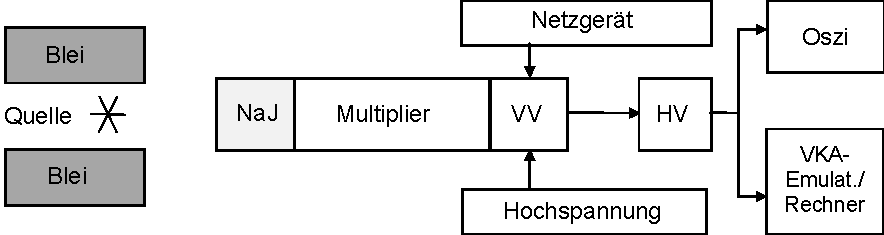
\includegraphics[width=.8\textwidth]{images/aufbau.pdf}
%\caption{Schematischer Aufbau des Versuchs \cite{wiki} mit NaJ-Detektor, VV-Vorverstärker, HV-Hauptverstärker, VKA-Vielkanalanalysator}
%\label{fig:aufbau}
%\end{figure*}


\section{Auswertung}

\subsection{Impulsformen}

Zu Beginn wurden die Impulsformen und -zeiten bestinmmt, um einen Eindruck über die Größenordnung der Totzeiten zu bekommen. Dazu wurde das Signal vor und nach 
Durchgang durch den Hauptverstärker mit dem Oszilloskop beobachtet. Die hierbei bestimmten Zeiten finden sich in Tabelle \ref{tab:zeiten}. 

\begin{table}
\centering
\begin{tabular}{ccc}
Detektor & Anstiegszeit & Abfallzeit \\
\hline
NaI VV & $700 \si{\nano \second}$ & $50 \si{\micro \second}$ \\
NaI HV & $700 \si{\nano \second}$ & $5 \si{\micro \second}$ \\
Ge  VV & $150 \si{\nano \second}$ & $300 \si{\micro \second}$\\
Ge  HV & $200 \si{\nano \second}$ & $6 \si{\micro \second}$ 
\end{tabular}
\caption{Anstiegs- und Abfallzeiten der benutztten Detektoren vor und nach dem Hauptverstärker}
\label{tab:zeiten}
\end{table}

Die Zeiten sind jedoch nur als ungefähre Werte zu sehen, da sich über das Oszilloskop nur schwer eine Zeit bestimmen lässt. Besonders die Abfallzeit ist nur 
eine grobe Schätzung. Es wird jedoch sofort deutlich, dass der Hauptverstärker die Abfall- und damit Totzeiten des Detektors signifikant verringert, 
im Fall des Szintillationsdetektors um ca. eine Größenordnung, im Fall von Germanium sogar um zwei. 

Die Anstiegszeiten sind im Fall des Halbleiter-Detektors deutlich kürzer, was zusammen mit der deutlich höheren Sensitivität eine viel bessere Auflösung zulässt. 
Dies ist auch in den folgenden Spektren zu sehen. 

Die Impulsformen wurden ebenfalls beobachtet und glichen bei beiden Detektoren in etwa denen in Abbildung \ref{fig:zeiten}. Es wurden Fotos der Impulsformen 
gemacht, allerdings sind bei diesen das Signals so schlecht zu sehen, dass nur die Skizze abgebildet ist.

\begin{figure}[h]
\centering
\begin{tikzpicture}
	\begin{axis}[
	width=.48\textwidth,
	ymin = -1.5,
	ymax = 1.5,
	xmin = 0,
	xmax = 10,
	xlabel={Zeit /a.u.},
	ylabel={Signal /a.u},
	]
	%\addplot[color = red] table {data/absorption_analytisch.txt};
	\draw [color=black, line width=.01pt ] ({axis cs:1.2,0}|-{rel axis cs:0,0}) -- ({axis cs:1.2,0}|-{rel axis cs:0,1});
	%\draw [color=black, line width=.01pt ] ({axis cs:556.942,0}|-{rel axis cs:0,0}) -- ({axis cs:556.942,0}|-{rel axis cs:0,1});
	\addplot[domain=0:5.5, color=blue]{sin((x)r)*e^(-.3*x)};
	\addplot[domain=5.5:10, color=blue]{-0.06*e^(-(x-6.3))};
	\addplot[domain=0:1.3, color=red]{-sin(((x+0.5))r)};
	\addplot[domain=1.3:10, color=red]{-1.06*e^(-0.3*(x-1))};
	\end{axis}
\end{tikzpicture}
\caption{Skizze der Impulsverläufe mit (blau) und ohne (rot) Hauptverstärker, die schwarze Linie markiert den ungefähren Übergang von Anstiegs- zu Abfallzeit}
\label{fig:zeiten}
\end{figure}

Aus dem Verlauf des Impulses ist zu schließen, dass der Hauptdetektor eine schwächere Dämpfung des Schwingungsprozesses den der Detektor durchläuft 
herbeiführt. Dadurch wird die Dämpfungskonstante des Prozesses verändert, was dazu führt, dass die Schwingung nun genau im aperiodischen Grenzfall 
abläuft. So wird die Zeit minimiert, bis der Schwinger oder Oszillator, in diesem Fall der Detektor, wieder zur Ruhe kommt. Dies minimiert die 
Totzeit und so können Ereignisse die dichter aufeinander folgen gemessen werden.

\subsection{Kalibrierung der Detektoren}

Um den Szintillationsdetektor zu kalibrieren bzw. zu wissen welcher Kanal des Vielkanalanalysators welcher Energie entspricht, wurden bei gleicher 
Einstellung des Hauptverstärkers Zerfälle verschiedener Energien gemessen. Die Messwerte sind in Tabelle \ref{tab:kalib_NaI} im Anhang aufgeführt. 


In Abbildung \ref{fig:kalib_NaI} sind alle für die Kalibrierung aufgenommen Daten zu sehen. Mithilfe von \cite{kohlrausch} konnten den Peaks die in Tabelle 
\ref{tab:kalib_NaI} ersichtlichen Energien zugeordnet werden. 

%\begin{figure*}[t]
%\centering
%\begin{tikzpicture}
%	\begin{axis}[
%	width=.8\textwidth,
%	height=.4\textwidth,
%	ymin = 0,
%	ymax = 450,
%	xmin = 0,
%	xmax = 8200,
%	xlabel={Kanal $\#$},
%	ylabel={Anzahl Ereignisse},
%	]
%	\addplot[color = red, thin] table {data/Kal_NaI_Co.txt};
%	\addplot[color = green, thin] table {data/Kal_NaI_Na.txt};
%	\addplot[color = blue, thin] table {data/Kal_NaI_Cs.txt};
%	\draw [color=black, line width=.01pt ] ({axis cs:5895,0}|-{rel axis cs:0,0}) -- ({axis cs:5895,0}|-{rel axis cs:0,1});
%	\draw [color=black, line width=.01pt ] ({axis cs:6705,0}|-{rel axis cs:0,0}) -- ({axis cs:6705,0}|-{rel axis cs:0,1});
%	\draw [color=black, line width=.01pt ] ({axis cs:3388,0}|-{rel axis cs:0,0}) -- ({axis cs:3388,0}|-{rel axis cs:0,1});
%	\draw [color=black, line width=.01pt ] ({axis cs:6396,0}|-{rel axis cs:0,0}) -- ({axis cs:6396,0}|-{rel axis cs:0,1});
%	\end{axis}
%\end{tikzpicture}
%\caption{Anzahl der Einfälle in Abhängigkeit vom Kanal für Cobal(rot), Cäsium(blau) und Natrium (grün) zur Kalibrierung des Analysators. Die schwarzen Linien 
%geben die Positionen der mit dem Messprogramm gefundenen und mit \cite{kohlrausch} identifizierten Peaks an}
%\label{fig:kalib_NaI}
%\end{figure*}

Mithilfe einer linearen Regression konnte eine Kalibrationsgerade gefunden werden.Für diese Kalibrierung wurde das Programm Mathematica 10 benutzt. 
So wurde die folgenden Kalibrationsgerade gefunden:
\begin{align}
(-24,9 \pm 3,4) + (0,2027 \pm 0,0007) \cdot x
\label{eq:kalib_NaI}
\end{align}


\begin{figure}[h!]
\begin{center}
\begin{tikzpicture}
\begin{axis}[
		width=.45\textwidth,
		ymin= 0,
		ymax= 1400,
		xmin = 0,
		xmax = 8000,
		xlabel={Kanal $\#$},
		ylabel={Enenergie/$\si{\kilo \electronvolt}$},
		]
\addplot[
   only marks, 
   error bars/.cd,
   x dir=both,
   x explicit,
   ]
table [ x index = {0},y index = {1}, x error index = {2} ] {data/Kal_NaI.txt};
\addplot[domain=0:8000] {-24.93 + 0.2027 * x}; 
\end{axis}
\end{tikzpicture}
\end{center} 
\caption{Kalibrationsgerade für den NaI-Szintillationsdetektor, Werte aus Tabelle \ref{tab:kalib_NaI}, Gerade mit Parametern aus Gleichung \ref{eq:kalib_NaI}}
\label{fig:Kalibrationsgerade_NaI}
\end{figure}

Die selbe Kalibrierung wurde für den Germanium-Detektor durchgeführt. Allerdings konnten hier aufgrund der höheren Sensitivität mehr Elemente zur Eichung benutzt 
werden. In Tabelle \ref{tab:Kalib_Ge} sind alle Energien und Kanäle aufgeführt, die Referenzwerte wieder aus \cite{kohlrausch}. Da für die Cobalt-Probe nur eine 
Langzeitmessung durchgeführt wurde, wird auf eine Darstellung aller Spektren in einer Abbildung verzichtet. 


Wieder wurde mit einer linearen Regression eine Kalibrationsgerade gefunden werden. Ebenfalls wurde das Programm Mathematica 10 benutzt. 
Die Parameter lauten wie folgend:
\begin{align}
(3,2 \pm 2,3) + (0,1839 \pm 0,0005) \cdot x
\label{eq:kalib_Ge}
\end{align}


\begin{figure}[h!]
\begin{center}
\begin{tikzpicture}
\begin{axis}[
		width=.45\textwidth,
		ymin= 0,
		ymax= 1400,
		xmin = 0,
		xmax = 8000,
		xlabel={Kanal $\#$},
		ylabel={Enenergie/$\si{\kilo \electronvolt}$},
		]
\addplot[
   only marks, 
   error bars/.cd,
   x dir=both,
   x explicit,
   ]
table [ x index = {0},y index = {1}, x error index = {2} ] {data/Kal_Ge.txt};
\addplot[domain=0:8000] {3.2 + 0.1839 * x}; 
\end{axis}
\end{tikzpicture}
\end{center} 
\caption{Kalibrationsgerade für den Halbleiterdetektor, Werte aus Tabelle \ref{tab:Kalib_Ge}, Gerade mit Parametern aus Gleichung \ref{eq:kalib_Ge}}
\label{fig:Kalibrationsgerade_Ge}
\end{figure}

Wie in Tabelle \ref{tab:kalib_fertig} zu sehen, ist die Kalibrierung gut, alle Werte für den Szintillationsdetektor sind gleich den Referenzwerten aus 
\cite{kohlrausch}. Für den Germanium Halbleiterdetektor sind fast alle Werte gleich den Literaturwerten, die drei energieärmsten Linien 
(Americium $60 \si{\kilo \electronvolt}$, Americium $26 \si{\kilo \electronvolt}$ und Barium $81 \si{\kilo \electronvolt}$) sind verträglich. Die Kalibrierung 
kann also ohne große Probleme verwendet werden, besonders im energiereichen Bereich stimmt sie sehr gut. Die Fehler wurden mit Gaußscher Fehlerfortpflanzung 
errechnet, wobei Eingangsfehler aus der Regressionsgeraden sowie aus den Messunsicherheiten stammen. Da das verwendete Messprogramm für die Full Width at 
Half Maximum (FWHM) für den Szintillationsdetektor teilweise offensichtlich falsche Werte lieferte, wurden hier von Hand bestimmte Schätzwerte benutzt. 
Die Messunsicherheit des Maximums der jeweiligen Gauss-Peaks wurden ebenfalls von Hand bestimmt: Dabei wurde der Unterschied des selbst bestimmten Maximums 
zum vom Programm bestimmten Maximum gewählt. 


\begin{table*}[t]
\centering
\begin{tabular}{cccccc}
Kanal & Energie (\cite{kohlrausch})/$\si{\kilo \electronvolt}$ & Energie /$\si{\kilo \electronvolt}$&$\Delta$ E /$\si{\kilo \electronvolt}$& FWHM 
/$\si{\kilo \electronvolt}$& $\Delta$ FWHM /$\si{\kilo \electronvolt}$\\
\hline
5895 & 1173,2 & 1170 & 10 & 50,68 & 0,87\\
6705 & 1332,5 & 1334,2 & 7,2 & 40,54 & 0,70\\
3388 & 661,6 & 661,8 & 5,1 & 50,66 & 0,87\\
6396 & 1274,5 & 1271,6 & 9,1 & 81,1 & 1,39\\
\hline
6377 & 1173,2 & 1175,9 & 4,2 & 2,464 & 0,035\\
7241 & 1332,5 & 1334,8 & 4,5 & 2,253 & 0,032\\
3599 & 664,6 & 665,1   & 3,2 & 1,857 & 0,026\\
6925 & 1274,5 & 1276,7 & 4,4 & 2,104 & 0,030\\
323 & 59,6 & 62,6      & 2,7 & 1,357 & 0,019\\
97 & 26,3 & 21,0       & 2,7 & 1,651 & 0,024\\
439 & 80,998 & 83,9    & 2,7 & 1,387 & 0,020
\end{tabular}
\caption{Vergleich der Literaturwerte der aufgenommenen Gammaenergien und der mit der Kalibrierung errechneten Werte für den NaI-Detektor (oben) und den Ge-Detektor 
(unten)}
\label{tab:kalib_fertig}
\end{table*}

Mithilfe dieser Eichung kann ebenfalls die Energie des in Abbildung \ref{fig:kalib_NaI} auffälig hervorragenden Peaks um Kanal Nummer 2976 auf ca. 
$518 \si{\kilo \electronvolt}$ bestimmt werden, was in etwa der Paarbildungsenergie entspricht. Da aber im Weiteren ein komplettes Spektrum mit besserer Statistik 
analysiert wird, wird hier auf weitere Auswertung des Spektrums des NaI-Detektors verzichtet. 

Wie man an den FWHM sehen kann, sind die Lebenszeiten der Zustände im NaI-Detektor signifikant länger als die im Ge-Detektor. Dies deckt sich mit den Werten aus 
Tabelle \ref{tab:zeiten}: Die Anstiegszeit im Halbleiterdetektor sind bedeutend kürzer (ca $ 70 \%$) als die im Szintillationsdetektor.  Das deutet auf eine 
längere Lebenszeit und damit eine größere Halbwertsbreite hin und erklärt die deutlichen Unterschiede in den FWHM der beiden Detektoren. 

\subsection{Bestimmung des Massenabschwächungskoeffizienten}

Im folgenden wurden die Massenschwächungskoeffizienten für Blei, Aluminium und Kupfer mithilfe der $1332 \si{\kilo \electronvolt}$-Cobalt-60-Linie bestimmt. Jede Messung 
wurde $180 \si{\second}$ durchgeführt, die Messwerte finden sich in den Tabellen \ref{tab:abs_blei}, \ref{tab:abs_alu} und \ref{tab:abs_kupfer} im Anhang. 
In Abbildung \ref{fig:absorption_alle} sind die Werte in einem halb-logarithmischen Plot zu sehen. Mit Formel \ref{eq:abs} kann der Absorptionskoeffizient $\mu$ 
bestimmt werden: 
\begin{align}
- \mu \cdot s &= \ln{\left( \frac{I(s)}{I_0} \right )} 
\end{align}
Da jedoch vergessen wurde, eine Nullmessung ohne Absorber durchzuführen, ist $I_0$ nicht bekannt. Mit dem Programm Mathematica 10 wird dennoch ein exponentieller 
Fit durchgeführt, dieser hat jedoch aufgrund der fehlenden Messung eine höhere Ungenauigkeit. 


\begin{figure}[h!]
\begin{center}
\begin{tikzpicture}
\begin{semilogyaxis}[
		width=.45\textwidth,
		ymin= 20000,
		ymax= 70000,
		xmin = 0,
		xmax = 25,
		xlabel={Materialdicke/$\si{\milli \meter}$},
		ylabel={Anzahl detektierter Zerfälle},
		]
\addplot[
   only marks, 
   color = blue,
   error bars/.cd,
   x dir=both,
   x explicit,
   y dir=both, 
   y explicit,
   ]
table [ x index = {0}, x error index = {1}, y index = {2}, y error index = {3}] {data/Abs_blei.txt};
\addplot[
   only marks, 
   color = red,
   error bars/.cd,
   x dir=both,
   x explicit,
   y dir=both, 
   y explicit,
   ]
table [ x index = {0}, x error index = {1}, y index = {2}, y error index = {3}] {data/Abs_alu.txt};
\addplot[
   only marks, 
   color = green,
   error bars/.cd,
   x dir=both,
   x explicit,
   y dir=both, 
   y explicit,
   ]
table [ x index = {0}, x error index = {1}, y index = {2}, y error index = {3}] {data/Abs_kupfer.txt};
\addplot[domain=0:25] {70492 * exp(-0.0564*x)}; 
\addplot[domain=0:25] {73251 * exp(-0.0161*x)}; 
\addplot[domain=0:25] {76816 * exp(-0.0493*x)}; 
\end{semilogyaxis}
\end{tikzpicture}
\end{center} 
\caption{Zählrate über Dicke des Absorbers, Daten aus \ref{tab:abs_blei} (blau, Blei), \ref{tab:abs_alu} (rot, Aluminium) und \ref{tab:abs_kupfer} (grün, Kupfer), 
y-Achse logarithmisch mit eingepassten Fits}
\label{fig:absorption_alle}
\end{figure}

Die mit Mathematica gefundenen Fits haben die in Tabelle \ref{tab:abs_parameter} stehenden Parameter. 
\begin{table}
\begin{tabular}{ccc}
Material & $I_0$ & $\mu$/$\nicefrac{1}{\si{\milli \meter}}$ \\
\hline 
Blei & 70261 $ \pm$ 1976 & 0,0564 $\pm$ 0,0026 \\
Aluminium & 73251 $\pm$ 4155 & 0,0161 $\pm$ 0,0041 \\
Kupfer & 75225 $\pm$ 5096 & 0,0472 $\pm$ 0,0044 \\
Kupfer & 76816 $\pm$ 967 & 0,0493 $\pm$ 0,0009
\end{tabular}
\caption{Parameter der exponentiellen Fits für die Bestimmung der Absorptionskoeffizienten}
\label{tab:abs_parameter}
\end{table}

Wird für Kupfer der Wert bei $17,5 \si{\milli \meter}$ und $15 \si{\milli \meter}$ nicht berücksichtigt, ergibt sich das in der Tabelle als viertes stehende Parameter-Set, 
welches einen deutlich kleineren Fehler zeigt und die anderen vier Punkte besser trifft. 
Die Werte für $I_0$ sind für die ersten drei Fits gleich. Somit scheint das nicht-aufnehmen dieses Wertes keinen großen Einfluss zu haben. Der alternativen 
Kupfer-Fit liegt allerdings außerhalb des einfachen Fehlerintervalls des Blei-Fits. Da hier aber die Berechnung von $\mu$ im Vordergrund steht, wird diesem Fakt 
keine weitere Bedeutung beigemessen. 

Um nun aus dem Absorptionskoeffizienten mit Formel \ref{eq:sigma} den totalen Wirkungsquerschnitt zu berechnen, wird die Atomdichte gebraucht. Diese errechnet sich 
folgendermaßen:
\begin{align}
n &= \frac{N}{V} = \frac{N \cdot \rho}{m} = \frac{N_A \cdot \rho}{m_T},
\end{align}
mit $n$ der Teilchendichte in $\nicefrac{1}{\si{\centi \meter}^3}$, $N$ der Teilchenanzahl, dem Volumen $V$, der Dichte $\rho$, der Avogadrokonstanten $N_A$ und der 
Teilchenmasse $m_T$. Die so errechneten Werte für den Totalen Wirkungsquerschnitt sind in Tabelle \ref{tab:querschnitte} einsehbar. Die Werte für die 
Teilchenmasse aus \cite{ciaaw}, die der Dichten aus \cite{greenwood}. 

\begin{table}[h]
\begin{tabular}{ccc}
Element & $n$/$\frac{1}{\si{\centi \meter}^3}$ & $\sigma_{tot}$/$\frac{1}{\si{\meter}^2}$ \\
\hline
Pb & $3,2965 \cdot 10^{22}$      & $(17,11 \pm 0,79) \cdot 10^{-28}$\\
Al & $2,5314 \cdot 10^{23}$ & $(0,63  \pm 0,16) \cdot 10^{-28}$\\
Cu & $8,4533 \cdot 10^{22}$    & $(5,83  \pm 0,11) \cdot 10^{-28}$\\
\end{tabular}
\caption{Wirkungsquerschnitte für Blei, Aluminium und Kupfer}
\label{tab:querschnitte}
\end{table}

Für die Wirkungsquerschnitte wurden keine Referenzwerte gefunden. Die Massenschwächungskoeffizienten $\sigma_m$ berechen sich mit $\nicefrac{\mu}{\rho}$. Die 
hier errechneten Werte finden sich in Tabelle \ref{tab:massen}. Referenzwerte aus \cite{NIST}. Da die Referenzwerte nur für Energien von $1250 \si{\kilo \electronvolt}$ 
und $1500 \si{\kilo \electronvolt}$ vorhanden sind, wurde, um einen Wert für die verwendete Cobalt-Linie zu bekommen, ein linearer Ausgleich zwischen diesen 
Punkten durchgeführt. Da der Verlauf des Massenschwächungskoeffizienten in Abhängigkeit der Energie jedoch nicht exakt ist, sind die Referenzwerte auch nicht exakt!

\begin{table}[h]
\begin{tabular}{ccc}
Element & $\sigma_m$ / $\frac{\si{\centi \meter}^2}{\si{\gram}}$ &  $\sigma_m$ / $\frac{\si{\centi \meter}^2}{\si{\gram}}$ \cite{NIST}  \\
\hline 
Pb & $0,0497 \pm 0,0023$    & $0,0061$ \\
Al & $0,060 \pm 0,015$ & $0,0056$ \\
Cu & $0,0552 \pm 0,0011$  & $0,0054$ \\
\end{tabular}
\caption{Massenschwächungskoeffizienten von Blei, Aluminium und Kupfer}
\label{tab:massen}
\end{table}

Wie zu sehen, sind die Werte für Kupfer und Aluminium gleich den Referenzwerte, die für Blei nicht. Da jedoch wie schon erwähnt der Referenzwert errechnet werden musste, 
und bei Blei der Verlauf am wenigsten linear ist, kann keine verbindliche Aussage über die Genauigkeit des Wertes getroffen werden. 

\subsection{Analyse eines Spektrums}

Über eine Zeitspanne von $4000 \si{\second}$ wurde ein Spektrum eines Cobalt-60-Strahlers aufgenommen, um Aussagen über auch weniger stark auftretende Effekte machen zu 
können. 

\subsection{Bestimmung der Konversionslinie}

Zeit: 180 s.



\section{Zusammenfassung}

\newpage
\bibliographystyle{unsrtnat}
\bibliography{gammabib}

\FloatBarrier
\begin{appendix}

\begin{table*}[h]
 \begin{tabular}{cccccccc}
Element & Energie /$\si{\kilo \electronvolt}$& Channel & Fehler & FWHM (PC) & FWHM (Mensch) & Net Area \\
\hline
Cobalt 60  & 1173,208 & 5895 & 42 & 30,36 & 250 & 21353 $\pm$ 1520 \\
Cobalt 60  & 1332,466 & 6705 & 21 & 147,24 & 200 & 14570 $\pm$ 1217 \\
Cäsium 137 &  661,638 & 3388 & 14 & 202,43 & 250 & 25487 $\pm$ 582 \\
Natrium 22 & 1274,511 & 6396 & 35 & 6,06 & 400 & 16739 $\pm$ 718 \\
 \end{tabular}
\caption{Messwerte zur Kalibrierung des Vielkanalanalysators für den NaI-Detektor, Messzeit je 120 $\si{\second}$}
\label{tab:kalib_NaI}
\end{table*}

\begin{table*}[h]
 \begin{tabular}{cccccccc}
Element & Energie /$\si{\kilo \electronvolt}$& Channel & Fehler & FWHM (PC) & FWHM (Mensch) & Net Area \\
\hline
Cobalt 60    & 1173,208 & 6377 & 7 & 13,40 & 28 & 62965 $\pm$ 486 \\
Cobalt 60    & 1332,466 & 7241 & 7 & 14,25 & 28 & 54430 $\pm$ 277 \\
Cäsium 137   &  661,638 & 3599 & 7 & 10,10 & 14 &  3189 $\pm$  61 \\
Natrium 22   & 1274,511 & 6925 & 7 & 11,44 & 14 &  2593 $\pm$  65 \\
Amercium 241 &   59,537 &  323 & 7 &  7,38 & 14 & 90468 $\pm$ 382 \\
Amercium 241 &   26,345 &   97 & 7 &  8,98 & 14 & 26518 $\pm$ 256 \\
Barium 133   &   80,998 &  439 & 7 &  7,54 & 14 &  7979 $\pm$ 196
\end{tabular}
\caption{Messwerte zur Kalibrierung des Vielkanalanalysators für den Germaniumdetektor, Messzeit je 180 $\si{\second}$, Cobalt-Peaks aus 4000 $\si{\second}$ 
Langzeitspektrum}
\label{tab:Kalib_Ge}
\end{table*}


\begin{table}[h]
\centering
\begin{tabular}{cc}
 Dicke & Zählrate  \\
 \hline 
 16,50 $\pm$ 0,06 mm & 27696 $\pm$ 1484  \\
 13,50 $\pm$ 0,05 mm & 33269 $\pm$ 1636  \\
 10,50 $\pm$ 0,04 mm & 38582 $\pm$ 1826  \\
  8,00 $\pm$ 0,03 mm & 43599 $\pm$ 1990  \\
  6,00 $\pm$ 0,02 mm & 50994 $\pm$ 2050  \\
\end{tabular}
\caption{Absorption Blei}
\label{tab:abs_blei}
\end{table}

\begin{table}[h]
\centering
\begin{tabular}{cc}
 Dicke & Zählrate \\
 \hline 
 21,00 $\pm$ 0,07 mm & 50276 $\pm$ 2177  \\
 18,00 $\pm$ 0,06 mm & 58059 $\pm$ 2091  \\
 15,00 $\pm$ 0,05 mm & 55323 $\pm$ 2255  \\
 12,00 $\pm$ 0,04 mm & 62792 $\pm$ 2185  \\
  9,00 $\pm$ 0,03 mm & 60228 $\pm$ 2357  \\
  6,00 $\pm$ 0,02 mm & 67514 $\pm$ 2283  \\
\end{tabular}
\caption{Absortion Alu}
\label{tab:abs_alu}
\end{table}

\begin{table}[h]
\centering
\begin{tabular}{cc}
 Dicke & Zählrate \\
 \hline
 22,00 $\pm$ 0,08 mm & 25753 $\pm$ 1583  \\
 20,00 $\pm$ 0,07 mm & 28991 $\pm$ 1620  \\
 17,50 $\pm$ 0,06 mm & 35525 $\pm$ 1611  \\
 15,00 $\pm$ 0,05 mm & 35221 $\pm$ 1851  \\
 12,00 $\pm$ 0,04 mm & 42395 $\pm$ 1890  \\
  9,00 $\pm$ 0,03 mm & 49374 $\pm$ 1995  \\
\end{tabular}
\caption{Absorption Kupfer}
\label{tab:abs_kupfer}
\end{table}
\end{appendix}

\begin{table*}[h]
\begin{tabular}{ccccccc}
 Element & 30-keV-Linie & FWHM & Net Area & 80-keV-Linie & FWHM & Net Area \\
 \hline
 Barium 133 pur & 1743 & 60,44 & 11170 $\pm$ 261 & 4593 & 54,53 & 6383 $\pm$ 215 \\
 Zinn (Sn)      & 1737 & 10,12 &  1928 $\pm$ 155 & 4594 & 56,06 & 5417 $\pm$  99 \\
 Antimon (Sb)   & 1754 & 19,06 &  2297 $\pm$ 159 & 4593 & 45,54 & 5333 $\pm$ 203 \\
 Tellur (Te)    & 1748 & 41,96 &  5342 $\pm$ 190 & 4591 & 34,96 & 5319 $\pm$ 201 \\
 Iod (I)        & 1742 & 47,86 &  4327 $\pm$ 178 & 4591 & 55,77 & 5584 $\pm$ 156 \\
\end{tabular}
\caption{Absorption für Konversionslinie}
\label{tab:konversion}
\end{table*}



\end{document}





